\documentclass{beamer}
\usepackage{tikz}
\usepackage{graphicx}
\usetheme{metropolis}

\title{Tetris Puzzle Solver}
\date{\today}
\author{James Fang, Miyuki Weldon, and Jonathan Lee}
\institute{EECS 106A at UC Berkeley}
\begin{document}
  \maketitle
  \begin{frame}{Goals}
    \begin{itemize}
      \item Develop puzzle board and pieces.
      \item Safely pick pieces from a table.
      \item Place pieces flush in a frame.
    \end{itemize}
  \end{frame}
  \begin{frame}{Design}
    \begin{figure}
      \includegraphics[height=0.85\textheight]{tiles-1}
      \hspace{0.5cm}
      \includegraphics[height=0.85\textheight]{tiles-2}
    \end{figure}
  \end{frame}
  \begin{frame}{Design}
    \begin{figure}
      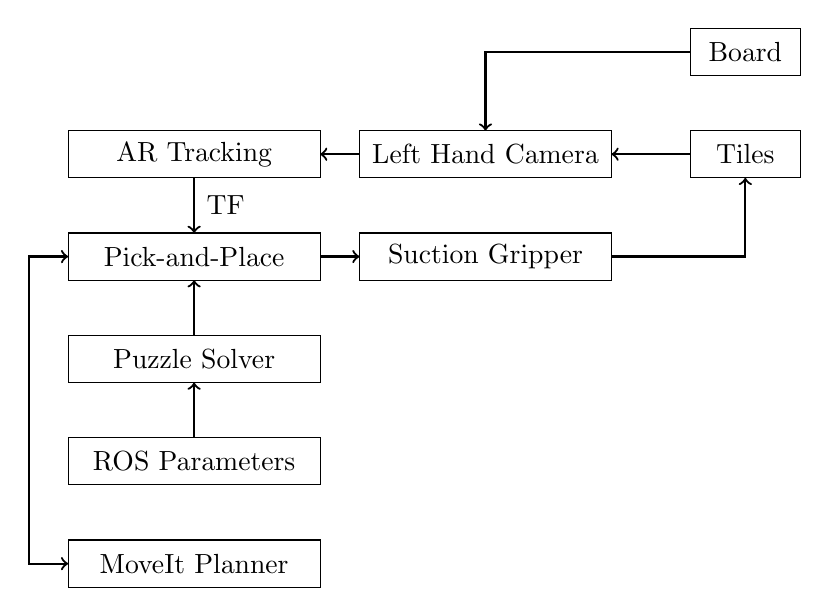
\begin{tikzpicture}
        \node at (0, 0) {Left Hand Camera};
        \node at (0, -1.3) {Suction Gripper};
        \node at (-3.7, 0) {AR Tracking};
        \node at (-3.7, -1.3) {Pick-and-Place};
        \node at (-3.7, -2.6) {Puzzle Solver};
        \node at (-3.7, -3.9) {ROS Parameters};
        \node at (-3.7, -5.2) {MoveIt Planner};
        \node at (-3.3, -0.65) {TF};
        \node at (3.3, 1.3) {Board};
        \node at (3.3, 0) {Tiles};

        \draw (-1.6, -0.3) rectangle (1.6, 0.3);
        \draw (-1.6, -1.6) rectangle (1.6, -1);
        \draw (-5.3, -0.3) rectangle (-2.1, 0.3);
        \draw (-5.3, -1.6) rectangle (-2.1, -1);
        \draw (-5.3, -2.9) rectangle (-2.1, -2.3);
        \draw (-5.3, -4.2) rectangle (-2.1, -3.6);
        \draw (-5.3, -5.5) rectangle (-2.1, -4.9);
        \draw (2.6, 1) rectangle (4, 1.6);
        \draw (2.6, -0.3) rectangle (4, 0.3);

        \draw[->, thick] (-1.6, 0) -- (-2.1, 0);
        \draw[->, thick] (-3.7, -0.3) -- (-3.7, -1);
        \draw[->, thick] (-2.1, -1.3) -- (-1.6, -1.3);
        \draw[->, thick] (-3.7, -2.3) -- (-3.7, -1.6);
        \draw[->, thick] (-3.7, -3.6) -- (-3.7, -2.9);
        \draw[<->, thick] (-5.3, -5.2) -- (-5.8, -5.2) -- (-5.8, -1.3) -- (-5.3, -1.3);
        \draw[->, thick] (1.6, -1.3) -- (3.3, -1.3) -- (3.3, -0.3);
        \draw[->, thick] (2.6, 0) -- (1.6, 0);
        \draw[->, thick] (2.6, 1.3) -- (0, 1.3) -- (0, 0.3);
      \end{tikzpicture}
    \end{figure}
  \end{frame}
  \begin{frame}{Challenges}
    \begin{itemize}
      \item Identifying tiles without AR tags (glare).
      \item Unstable AR marker estimates. Unknown table height.
      \item Tile types share an AR marker ID.
      \item Bad grasps (depressions on tags).
    \end{itemize}
  \end{frame}
  \begin{frame}{Improvements}
    \begin{itemize}
      \item Adding two AR markers per tile for greater pose stability.
      \item Placing tags away from the tile center-of-mass.
      \item Assigning unique AR tags.
    \end{itemize}
  \end{frame}
\end{document}
